\documentclass[12pt]{article}
\usepackage[utf8]{inputenc}
\usepackage[english,russian]{babel}
\usepackage[OT1]{fontenc}
\usepackage{amsfonts, amsmath, amsthm, amssymb}
\usepackage[left=1cm,right=1cm,top=1cm,bottom=2cm]{geometry}
\usepackage{paralist}
\usepackage{graphicx}
\usepackage{wrapfig}
\usepackage{mathtools}
\usepackage{comment}

\def\frac#1#2{\mathchoice{#1\over#2}{\hbox{\small$#1$}\over\mathstrut\hbox{\small$#2$}}{#1\over#2}{#1\over#2}} 

\newcounter{problem}
\newcommand{\problem}{\par \bigskip \refstepcounter{problem}%
\textbf{№\arabic{problem}.} }

\def \Problem#1{\par \bigskip \textbf{Problem №{#1}. }}
\def \solution{\par \bigskip \textbf{Solution. }}
\def \solutionI{\par \bigskip \textbf{First solution. }}
\def\solutionII{\par \noindent \textbf{Second solution. }}
\def\solIII{\par \noindent \textbf{Third solution. }}
\def\lemmaI{\noindent \textbf{Lemma. }}
\def\lemma#1{\noindent \textbf{Lemma {#1}. }}
\def\proof{\par \noindent \textbf{Proof. }}

\def \answer{\par \bigskip \textbf{Answer. }}
\def \marking{\par \bigskip \textbf{Marking scheme. }}

\DeclareRobustCommand{\divby}{%
  \mathrel{\text{\vbox{\baselineskip.65ex\lineskiplimit0pt\hbox{.}\hbox{.}\hbox{.}}}}%
}

\begin{document}

\centerline{\sc \textbf{XXI Silk Road Mathematical Competition}}

\centerline{\sc \textbf{March 2022}}

\bigskip
\hrule
\bigskip

\textsl{\textbf{Attention!} 
We ask you not to \textbf{disclose} these problems and not to discuss them publicly (especially through Internet) before May 25, 2022.}

\bigskip

\centerline{\sc \textbf{Solutions and marking schemes}}

\bigskip

\bigskip
\Problem{1} Convex quadrilateral $ABCD$ is inscribed in circle $\omega$. Rays $AB$ and $DC$ intersect at $K$. $L$ is chosen on the diagonal $BD$ so that $\angle BAC = \angle DAL$. $M$ is chosen on the segment $KL$ so that $CM \parallel BD$. Prove that the line $BM$ touches $\omega$. \textit{(Kungozhin~M.)}

\begin{wrapfigure}{r}{0.3\textwidth}
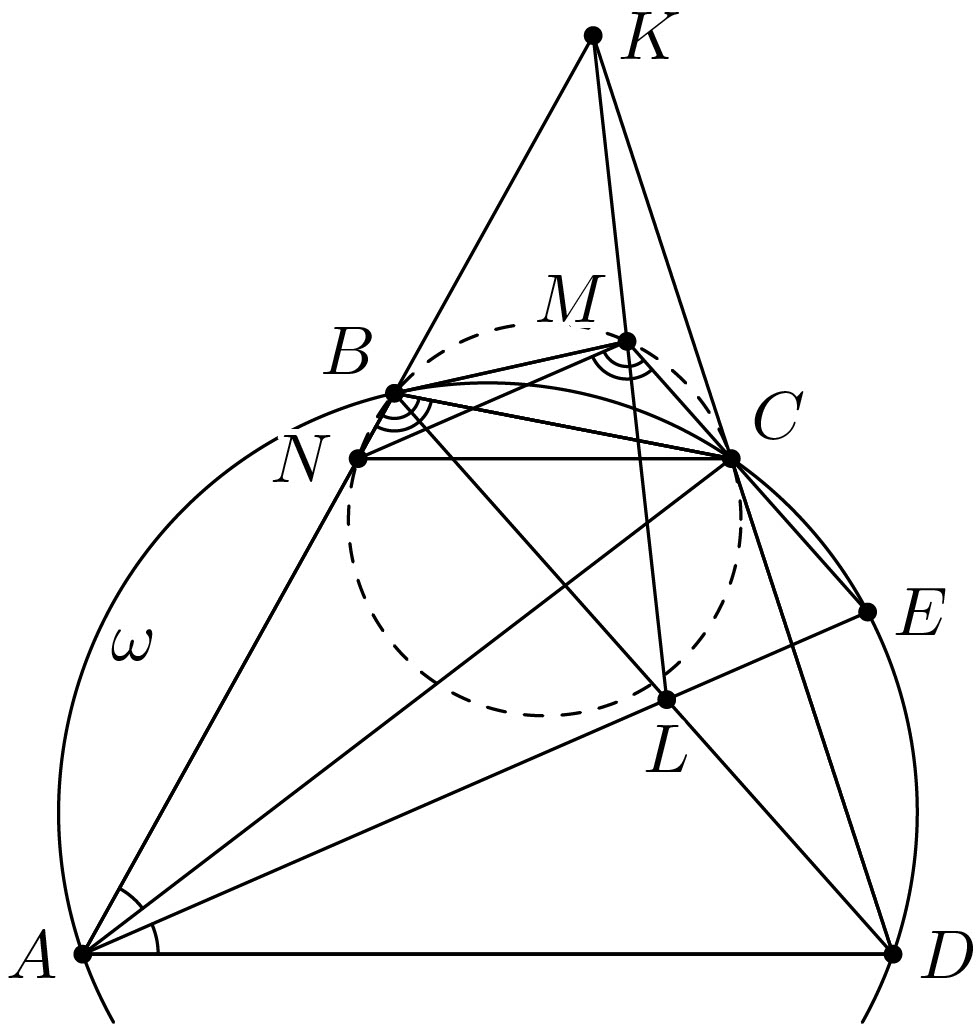
\includegraphics[width=0.3\textwidth]{img_1.jpg}
\end{wrapfigure}

\solutionI Let $N$ be a point on the line $AK$ so that $MN \parallel AL$. Since
$\dfrac{CM}{DL} = \dfrac{NM}{AL} = \dfrac{KM}{KL}$ and $\angle CMN = \angle DLA$, it follows that $K$ is a center of homothety which sends $\triangle CMN$ into similar $\triangle DLA$. On the other hand, $\triangle DLA$ is similar to $\triangle CBA$ because $\angle DAL = \angle BAC$ and $\angle ADL = \angle ACB$. Consequently, $\angle(BN, BC) = \angle(MN, MC)$, and thus points $N, B, M, C$ are cyclic. Therefore, $\angle CBM = \angle CNM = \angle CAB$ from which it follows that $BM$ touches $\omega$.

\solutionII For this solution we need the following theorem.

\textbf{Pascal's theorem.} Points $A, B, C, D, E, F$ (not necessarily in this order) lie on some circle. Then the intersections of the lines $AB$ and $DE$, $BC$ and $EF$, $CD$ and $FA$ lie on a straight line.

Back to the problem. Let $E$ be the second intersection of the line $AL$ and $\omega.$ Define $\ell_b$ as a tangent line to $\omega$ at $B$. Let's apply Pascal's theorem on points $B, B_1, A, E, C, D$ (here $B_1$ coincides with $B$) and pairs of lines $(BB_1, EC)$, $(B_1A, CD)$, $(AE, DB).$ These pairs of lines coincide with pairs of lines $(\ell_b, EC)$, $(BA, CD)$, $(AE, DB)$. Then from Pascal's theorem, the straight line connecting $K = BA \cap CD$ and $L = AE \cap DB$ will also contain $\ell_b \cap EC$. Since $M = EC \cap KL$, it follows that $BM$ touches $\omega$, as desired.

\marking
\\ 1. Unfinished bashing \\(using coordinates, complex numbers, vectors, trigonometry, etc.): 
\dotfill \textbf{0 points}
\\ 2. Proof of the similarity $\triangle ADL \sim \triangle ACB$: \dotfill \textbf{1 points}
\\ 3. Proof of the similarity $\triangle CMN \sim \triangle DLA$: \dotfill \textbf{3 points}
\\ 4. It is proven that the points $N, B, M, C$ are cyclic: \dotfill \textbf{2 points}
\\ 5. It is proven that the points $M, C, E$ lie on a straight line (doesn't add up with 2): \dotfill \textbf{1 points}
\\ 6. Application of Pascal's theorem without any details (depending on which collection of points to apply): \dotfill \textbf{0 points}
\\ 7. Application of Pascal's theorem on wrong collection of points: \dotfill \textbf{0 points}
\\ 8. Application of Pascal's theorem on the right collection of points without details on the pairs of lines: \dotfill \textbf{2 points are deducted}
\\ 9. For the non-consideration of all possible configurations of points no points are deducted.

\newpage
\Problem{2} Distinct positive integers $A$ and $B$ are given. Prove that there exist infinitely many positive integers that can be represented both as $x_1^2 + Ay_1^2$ for some positive coprime integers $x_1$ and $y_1$, and as $x_2^2 + By_2^2$ for some positive coprime integers $x_2$ and $y_2$.
\textit{(Golovanov A.S.)}

\solution Without loss of generality $A > B$.

Choose an arbitrary prime $p > 2$ and let's find $x_1$ and $x_2$ so that 

$$x_1^2 + A(2p)^2 = x_2^2 + B(2p)^2,$$

Hence, $x_2^2 - x_1^2 = 4Cp^2$ where $C = A - B$. Set $x_1 = Cp^2 - 1$ and $x_2 = Cp^2 + 1$. If $x_1$ and $x_2$ are both odd, then they are both coprime with $y = 2p$, and we have $x_1^2 +  Ay^2 = x_2^2 + By^2$. If they are both even , then $x_1\over 2$ and $x_2 \over 2$ are both coprime with $y = p$, and we have $\left({x_1\over 2}\right)^2+Ay^2=\left({x_2\over 2}\right)^2+By^2$.

The number to which we have found two such forms will be not less than $p^2$, thus proving there are infinitely many such numbers.

\marking
\\ 1. It is proven that if $x_1 = Cp^2 - 1$ and $x_2 = Cp^2 + 1$ are both odd, then the number $x_1^2 + Ay^2 = x_2^2 + By^2$ satisfies the problem conditions, where $y = 2p$: \dotfill \textbf{5 points}.
\\ 2. It is proven that if $x_1 = Cp^2 - 1$ and $x_2 = Cp^2 + 1$ are both even, then the number $\left(\frac{x_1}{2}\right)^2+Ay^2=\left(\frac{x_2}{2}\right)^2+By^2$ satisfies the problem conditions, where $y = p$: \dotfill \textbf{5 points}
\\ 3. It is proven that infinitely many such numbers exist (only if 1. or 2. is present): \dotfill \textbf{1 point}
\\ 4. Points for 1. and 2. do not add up.
\\ 5. If 1. and 2. are both present: \dotfill \textbf{plus 1 point}

\Problem{3} 
In an infinite sequence $\{\alpha\}$, $\{\alpha^2\}$, $\{\alpha^3\}$, \dots there are only finitely many distinct values. Show that $\alpha$ is an integer. ($\{x\}$ denotes the fractional part of $x$, i.e. $\{x\} = x - [ x ]$, where $[ x ]$ is the greatest integer not greater than $x$.) \textit{(Golovanov A.S.)}

\solution 
\textit{Step 1.} We show that there is a positive integer $l$ s.t. $\alpha^l$ is rational. Say the sequence is of length $k-1$. For any positive integer $n$ we the sequence $\{\alpha^{nk}\}$, 
$\{\alpha^{nk+1}\}$, \dots, $\{\alpha^{nk+k-1}\}$ contains two equal elements. Hence, there are infinitely many pairs $i$, $j$,
$0<i-j<k$, such that $\{\alpha^i\}=\{\alpha^j\}$, i.e. $\alpha^j(\alpha^{i-j}-1)$ is an integer. Since there are finitely many possible values of $i-j$, at least one of them occurs infinitely often. So we can find $m$ such that $\alpha^j(\alpha^m-1)$ is an integer for infinitely many $j$. We can divide two such numbers to get $\alpha^l$ is rational for some positive integer $l$.

\textit{Step 2.} Conclusion. Now if $\alpha^l$ is not an integer, say, is equal to $\frac{a}{b}$ for $b>1$, gcd$(a,b)=1$, then $\{\alpha^{ln}\}$ is an irreducible fraction with denominator $b^n$. This is true for any $n$ so we get infinitely many values, contradiction. So $\alpha^l$ is an integer. If $\alpha$ is irrational, then $\alpha^{nl+1}=\alpha^{nl}\cdot\alpha$ is irrational for any natural $n$ and have distinct fractional parts (Indeed, $\alpha^{il+1}-\alpha^{jl+1}=\alpha (\alpha^{il}-\alpha^{jl})$ cannot be an integer). This contradicts finiteness as well. Thus $\alpha$ is rational, and similar to above we can conclude it is an integer.


\marking
\\ 1. Proof of step 1: \dotfill \textbf{ 4 points}
\\ 2. Attempt to construct $m$ such that $\alpha^j(\alpha^m-1)$ is an integer for two different $j$'s: \dotfill \textbf{ 1 point}
\\ 3. Found $i$ and $j$ such that $\{\alpha^i\}=\{\alpha^j\}$ and $|i-j|$ is bounded above by some constant which might depend on $k$ (and not on $i$ or $j$): \dotfill \textbf{2 points}
\\ 4. Proof of step 2, i.e. that if $\alpha^l$ is rational for some $l$, then $\alpha$ is an integer: \dotfill \textbf{ 2 points}
\\ 5. Proof of the fact that $\alpha$ is either irrational or an integer (or equivalent): \dotfill \textbf{ 1 points}
\\ 6. Point 1 does not add up with points 2 or 3, point 4 does not add up with point 5.

\newpage
\Problem{4} In a language, an alphabet with 25 letters is used; \emph{words} are exactly all sequences of (not necessarily different) letters of length $17$. Two ends of a paper strip are glued so that the strip forms a ring; the strip bears a sequence of $5^{18}$ letters. Say that a word is \emph{singular} if one can cut out a piece bearing exactly that word from the strip, but one cannot cut out two such non-overlapping pieces. It is known that one can cut out $5^{16}$ non-overlapping pieces each containing the same word. Determine the largest possible number of singular words. \textit{(Bogdanov I.)}

\answer $2\cdot 5^{17}$.

\solution Let the alphabet consist of letters $a_1,a_2,\dots,a_{25}$. By a \emph{piece} we always mean a piece of the strip containing exactly 17 consecutive letters; different pieces may contain the same word. Say that a piece is \emph{singular} if the word it contains is such.

\medskip
We start with constructing an example containing $N=2\cdot 5^{17}$ singular words. Define a word $W=a_1a_2\dots a_{17}$; this will be the word having $k=5^{16}$ non-overlapping copies on the strip. There exist exactly $25^8=k$ possible 8-letter sequences, consisting of letters $a_{18}, a_{19}, \ldots, a_{25}$; put them onto the strip in an arbitrary order, separating each two sequences by an instance of~$W$. Each segment of the strip containing one 8-sequence mentioned above (and no other letters) will be referred to as a \emph{part}. Notice that the strip contains exactly $(8+17)k=5^{18}$ letters.

Clearly, the obtained strip contains $k$ non-overlapping copies of~$W$. Now we show that any piece containing a whole part is singular --- moreover, that the word it contains is met on no other piece. Since a part can be situated in a piece at 10 different positions (starting from the 1-st, from the 2-nd, \dots, or from the 10-th letter of a piece), we will get that there are at least  $10\cdot 5^{16}=N$ singular words.

\smallskip
Consider an arbitrary piece $p$ containing a word $P$. Either this piece contains a unique nonempty prefix which coincides with some suffix of $W$, or there is no such prefix --- only in this case we will say that such prefix is empty. Let $b$ be the length of the defined prefix. Define similarly a suffix of $P$ which coincides with a prefix of~$W$, and denote its length by~$e$. Notice that the defined prefix and suffix do not overlap whenever $P\neq W$ (if $P=W$, we have $b=e=17$).

If the piece contains no whole part, then $\max\{b,e\}>9$. If the piece contains a part, then $b+e=9$ and $0 \le b, e \le 9$. Thus, piece $p$ contains a part if and only if $\max\{b,e\}\leq 9$, and in this case the position of the part at $P$ (and hence the position of $p$ at the strip) is uniquely determined. Therefore, in this case $P$ is met only on piece $p$, so this piece is singular. We have proven that the constructed example works.

\medskip
It remains to prove that the number of singular words cannot exceed $N$. Enumerate the positions in the strip successively by $1,2,\dots,5^{18}$ (the numeration is cyclic modulo $5^{18}$). Let $p_i$ denote the piece starting at position $i$, and let $P_i$ be the word on that piece. Let $n_1,\dots,n_k$ be positions such that the pieces $p_{n_1}$, $p_{n_2}$, \dots, $p_{n_k}$ are pairwise disjoint and contain the same word $W$ (from the problem statement). Clearly, those pieces are not singular.

For $i=1,2,\dots,8$ and  $1\leq s\leq k$, we say that a piece $p_{n_s+i}$ is a \emph{rank $i$ follower}, while $p_{n_s-i}$ is a \emph{rank $i$ predecessor}. All these pieces (followers and predecessors) are distinct; moreover, followers of a fixed rank are pairwise disjoint, and the same holds for predecessors. We will show that \textit{among $8\cdot 5^{16}$ followers of all ranks, at most $5^{16}$ pieces are singular} (we will call this statement a \textit{quoted claim} in the future); by symmetry, the same bound holds for predecessors. This will yield that there are at least $5^{16}+7\cdot 5^{16}+7\cdot 5^{16}=3\cdot 5^{17}$ non-singular pieces, which implies the desired bound.

\smallskip
Thus, we are left to prove the claim quoted above. For any rank~$i$ follower $p_{n_s+i}$ define its \emph{tail}
%$T_{s,i}$
as its suffix of length~$i$ (the tail consists of all letters which do not lie in $p_{n_s}$; we regard a tail as a sequence of letters). We show by induction on $m=0,1,\dots,8$ that for every sequence $U$ consisting of $(8-m)$ letters, there are no more than $25^m$ followers whose tails contain $U$ as a prefix. The desired claim is obtained by setting $m=8$.

The base case $m=0$ is obvious: if a follower with tail $U$ is singular, then there is only one such follower. Let us perform the inductive step. If there is no singular follower whose tail is $U$, then every singular follower's tail starting with $U$ starts in fact with some word of the form $Ua_i$. For every $i=1,2,\dots,25$, there are at most $25^{m-1}$ such followers, by the inductive hypothesis. So the total number of such followers does not exceed  $25\cdot 25^{m-1}=25^m$, as desired.

Finally, if there is a singular follower $P_{n_s+8-m}$ whose tail is $U$, then such follower is unique. Therefore, all followers of larger ranks whose tails start with $U$ correspond to the same copy $p_{n_s}$ of~$W$. Then the number of such followers (including $P_{n_s+8-m}$ itself) is at most $m+1\leq 25^m$, as desired again. The claim, and the bound, are proven.

\medskip
\textbf{Remark.} We present a shorter (yet more ideological) proof of the quoted claim on the number of singular followers. Say that a singular follower's tail $T$ is \emph{minimal} if none of its proper prefixes is a singular follower's tail. In particular, no minimal tail can be a proper prefix of other minimal tail.

For every minimal tail $T$ let us write down all $8$-letter sequences starting with $T$; if the length of $T$ is $d$, then the number of such sequences is $25^{8-d}$. No sequence could be written down twice; therefore, if there are $M$ minimal tails of lengths $d_1,\dots,d_M$, then
$$
  \sum_{i=1}^M 25^{8-d_i}\leq 25^8.
$$

On the other hand, each singular follower's tail has a prefix which is a minimal tail. For a minimal tail $T$ of length~$d$, there are at most $9-d$ singular followers whose tails start with $T$ --- at most one per tail's length. Therefore, the number of singular followers does not exceed 
$$
  \sum_{i=1}^M (9-d_i)\leq \sum_{i=1}^M 25^{8-d_i}\leq 25^8,
$$
since $9-d\leq 25^{8-d}$ for all $d=1,2,\dots,8$.


\marking
\\ 1. An example with $2\cdot 5^{17}$ singular words: \dotfill \textbf{2 points}
\\ 2. Proof of the example's correctness: \dotfill \textbf{1 point}
\\ 3. Proof of the fact that the answer is not greater than $2\cdot 5^{17}$: \dotfill \textbf{4 points}
\\ 4. Formulation of the quoted claim: \dotfill \textbf{1 point}
\\ 5. The points for 3. and 4. do not add up.

\end{document}
